%% The first command in your LaTeX source must be the \documentclass command.
\documentclass[sigchi]{acmart}

%% For page numbers! Yay!
\settopmatter{printfolios=true}

%%
%% Remove the ACM copyright information. Found on:
%% https://tex.stackexchange.com/questions/346292/how-to-remove-conference-information-from-the-acm-2017-sigconf-template
% Removes citation information below abstract
\settopmatter{printacmref=false}
% removes footnote with conference information in first column
\renewcommand\footnotetextcopyrightpermission[1]{} 

%% Please use this for your title. We use the long version for the title on the
%% first page and the shorter version for the running page header on the right.
\newcommand{\myLongTitle}{Heuristic evaluation of interactive machine learning systems} %% @TODO
\newcommand{\myShortTitle}{HE of IML systems} %% @TODO

%% \BibTeX command to typeset BibTeX logo in the docs
\AtBeginDocument{%
  \providecommand\BibTeX{{%
    \normalfont B\kern-0.5em{\scshape i\kern-0.25em b}\kern-0.8em\TeX}}}

%%
%% Remove copyright note by ACM: Found on:
%% https://tex.stackexchange.com/questions/21536/how-to-remove-the-copyright-box-on-a-paper-that-uses-the-acm-sig-alternate-cls-c
\setcopyright{none} 

%% own package usages

%%
%% end of the preamble, start of the body of the document source.
\begin{document}

%%
%% The "title" command will get the content of "myLongTitle".
\title{\myLongTitle{}}

%% The "subtitle" command is used for the course title and will change
%% every semester.
\subtitle{Proseminar "Interactive Intelligent Systems", Winter Term, 2020/21}

%%
%% The "author" command and its associated commands are used to define
%% the author and affiliation.
\author{Jan Ole Zabel}
\affiliation{%
  \institution{Freie Universität Berlin}
  \city{Berlin}
  \country{Germany}
}
\email{jan.zabel@fu-berlin.de}

%%
%% By default, the author name and the "short title" of the document is
%% printed in the page headers. As the full name and the title is sometime very
%% long and stuff might overlap, please use a short version of your name here.
\renewcommand{\shortauthors}{J. Zabel - \myShortTitle{}}

%%
%% This snippet is used a the page header on the outer. This should be changes
%% every semester.
\acmConference[Proseminar "Interactive Intelligent Systems"]{PS IIS}{Winter Term}{2020/21}

%%
%% The abstract is a short summary of the work to be presented in the
%% article.
\begin{abstract}
Interactive Machine Learning enables end-users to design machine learning models. This completely new mode of human-computer interaction requires a high level of usability, which has naturally to be evaluated. The Heuristic Evaluation is a method for analysing software usability, which only needs adjusted heuristics to be applied to IML. On the other hand, there exists a significant but not total lack of research within these combination.
\end{abstract}

%%
%% Keywords. The author(s) should pick words that accurately describe
%% the work being presented. Separate the keywords with commas.
\keywords{human computer interaction, usability analysis, heuristic evaluation, interactive machine learning}

%%
%% This command processes the author and affiliation and title
%% information and builds the first part of the formatted document.
\maketitle

\pagenumbering{arabic}

%%
%% Add a table of contents to this ACM template
%% Removed "Abstract", "ACK", and "References" from TOC (2401 in acmart.cls)
%% Removing the Contents headline from the TOC!
\let\oldaddcontentsline\addcontentsline
\newcommand{\stoptocentries}{\renewcommand{\addcontentsline}[3]{}}
\newcommand{\starttocentries}{\let\addcontentsline\oldaddcontentsline}

\stoptocentries% Stop adding content to the ToC
\tableofcontents
\starttocentries% Resume adding content to the ToC

\section{Introduction}
Since software has started being developed, there has been a natural interest in measuring its usability, as its usage by humans is an integral part of every software. Non-usable software is worthless in the best case, and dangerous in the worst. However, most methods for evaluating usability are made for traditional software without AI abilities. Thus, for intelligent systems, these methods have to be re-evaluated.

This is especially true for Interactive Intelligent Systems (IIS). A special case within these is the interactive machine learning (IML), where the user's feedback is the most integral part. A user trains a model who is not necessarily an expert on the field. This is accomplished through the smart use of visualizations and the user's ability to evaluate the model's decisions. The usability is the most important thing here, although it may be difficult to measure by traditional methods.

Heuristic evaluation \cite{heureval1990} is a usability analysis method that is comparably easy to perform. By aggregating multiple evaluator's input after a semi-formal review, many usability problems can be found.

\section{Interactive Machine Learning}
As AI-driven software becomes more and more important, the same applies for the creation and adaptation of machine-learning models. Interactive Machine Learning (IML) enables "everyday users to interactively explore the
model space through trial-and-error and drive the system towards an
intended behavior, reducing the need for supervision by practitioners"\cite{reviewiml2018}.

The method is done by providing users well visualized feedback on the current performance of a model, and after getting user input back, automatically adjust the model. This can be seen as a feedback loop, and is visualized in figure \ref{fig:iml}.

Many machine-learning approaches benefit from a human in the loop\cite{humankernel2015}, which is also shown by empirical data \cite{imlexp2018}, although IML puts a constraint on the algorithms that can be used with this approach\cite{iml2003}. For instance, many machine learning algorithms optimise on the time the classification takes, but take a long time to train. However, the training should be done in nearly real-time to be an interactive process. This means the usage of fast training algorithms is important. "This  allows the interactive cycle to be iterated quickly so it can be done more frequently."\cite{iml2003}.
\begin{figure*}[h]
  \centering
  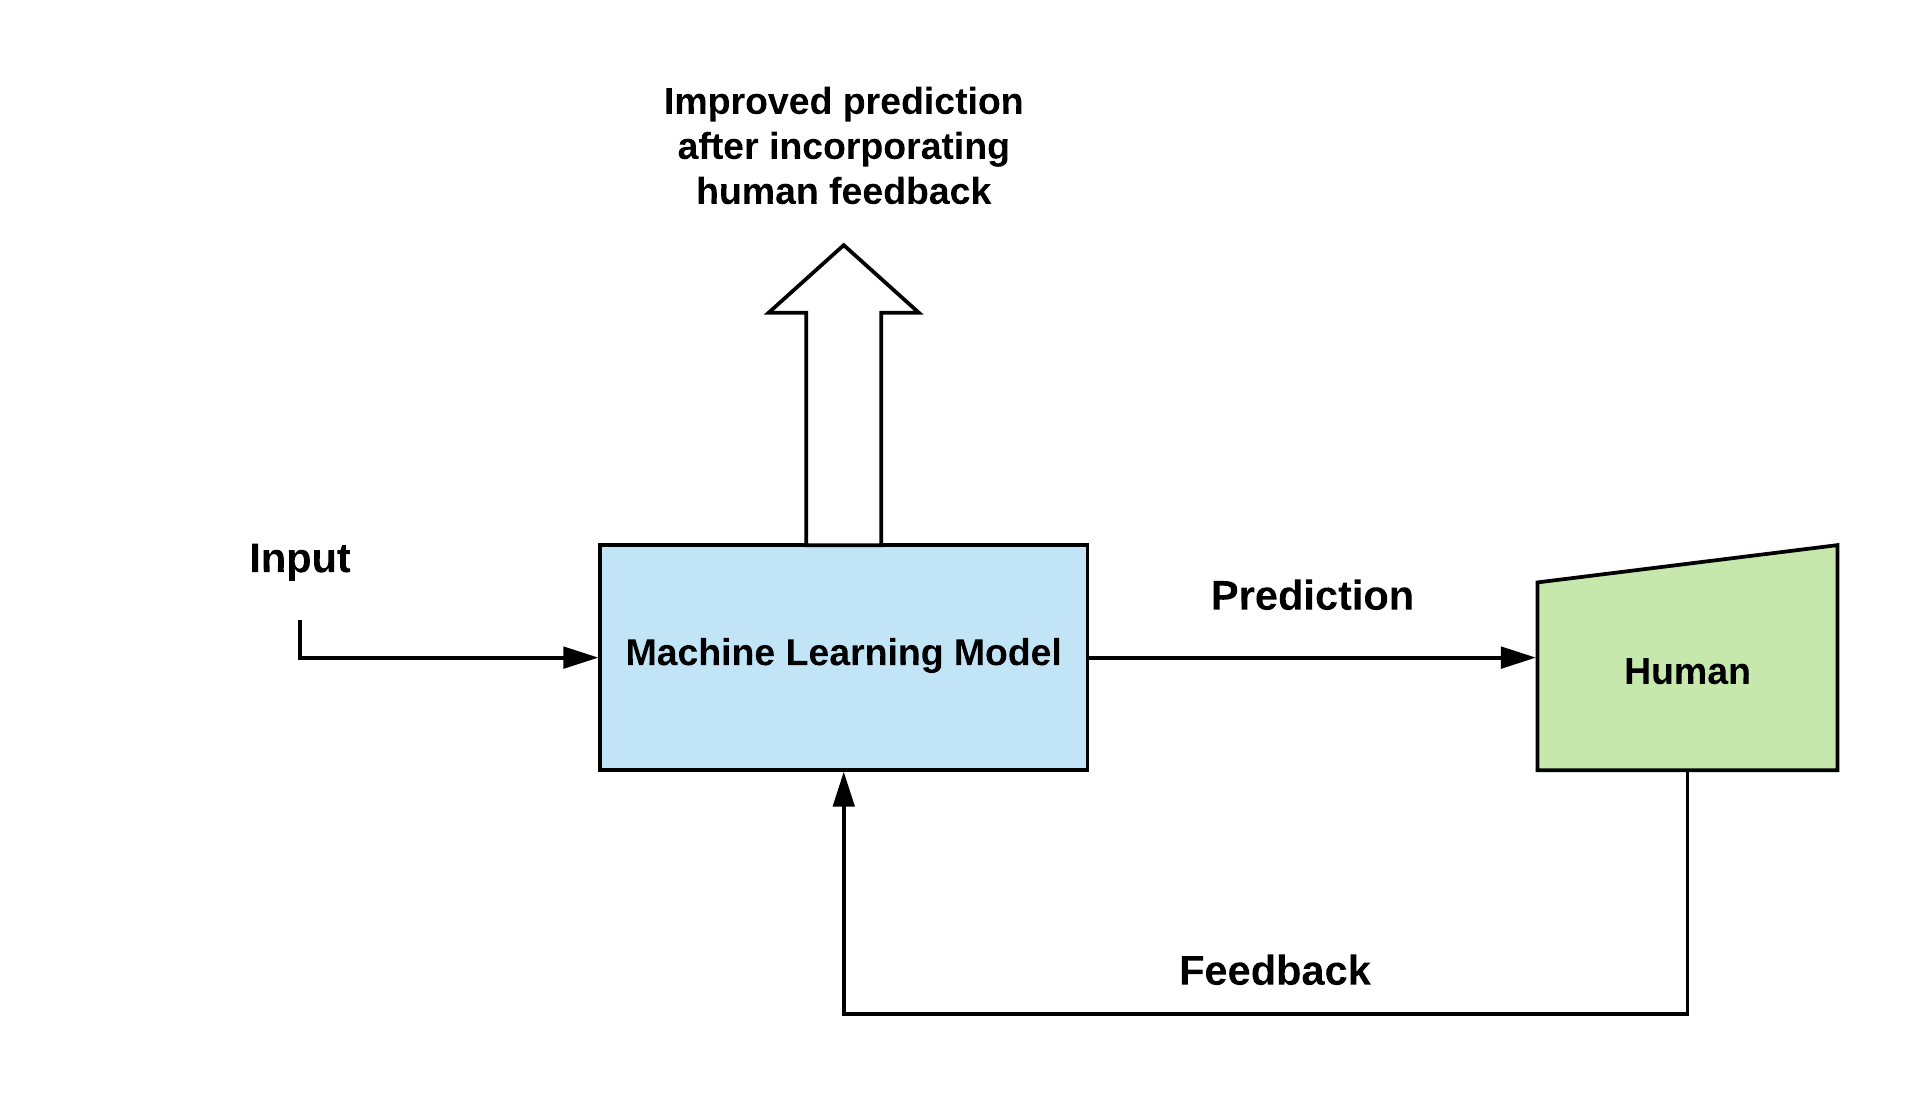
\includegraphics[width=0.8\linewidth]{iml-scheme}
  \caption{Scheme of the IML approach\cite{whatiml2018}}
  \label{fig:iml}
\end{figure*}

\section{Heuristic Evaluation}
The heuristic evaluation is one of the most relied upon method for measuring usability aspects of software. In their early empirical review of this method, \citeauthor{heureval1990} state:
"There are basically four ways to evaluate a user interface: Formally by some analysis technique, automatically by a computerized procedure, empirically by experiments with test users, and heuristically by simply looking at the interface and passing judgement according to ones own opinion."

\subsection{Conducting heuristic evaluation}

\citeauthor{heureval1990} also provide a definition of heuristic evaluation: "Heuristic evaluation is done by looking at an interface and trying to come up with an opinion about what is good and bad about the interface."~\cite{heureval1990} In practice, this can be done also with a specification of a user interface, or with screenshots of the interface. Therefore, it is not necessary to have a finished prototype.

Best, this  evaluation is done according to a preferably simple set of usability rules, which are called the heuristics. Nielsen and Molich set up nine basic rules which define what a usability problem actually should violate (table \ref{tab:9heur}). Later, Nielsen updated this set to a quite different list of ten heuristics (table \ref{tab:10heur}).

As a result of this process, a list of problems emerges.

\begin{table}
  \caption{Nine basic rules for evaluation}
  \label{tab:9heur}
  \begin{tabular}{ccl}
    \midrule
    Simple and natural dialogue\\
    Speak the user’s language\\
    Minimize user memory load\\
    Be consistent\\
    Provide feedback\\
    Provide clearly marked exits\\
    Provide shortcuts\\
    Good error messages\\
    Prevent errors\\
  \bottomrule
\end{tabular}
\description{\citeauthor{heureval1990} 1990~\cite{impdialog1990}~\cite{heureval1990}}
\end{table}

\begin{table}
  \caption{Updated ten other heuristics for evaluation}
  \label{tab:10heur}
  \begin{tabular}{ccl}
    \midrule
    Visibility of system status \\
    Match between system and the real world \\
    User control and freedom \\
    Consistency and standards \\
    Error prevention \\
    Recognition rather than recall \\
    Flexibility and efficiency of use \\
    Aesthetic and minimalist design \\
    Help users recognize, diagnose, and recover from errors \\
    Help and documentation \\
  \bottomrule
\end{tabular}
\description{\citeauthor{he1994} 1994~\cite{he1994}}
\end{table}


\subsection{Reasons to use heuristic evaluation}
The method is used for a number of benefits.

Firstly, it is organisationally easy to do.  It does not have a long list of dependencies. It can be done at any point in time in the development process, without much communication needed to other teams or processes.~\cite{evalmethods2018}

Secondly, it is costly inexpensive. It does not require a large number of experts or time, and these do not even have to be usability experts.~\cite{evalmethods2018}

There are other benefits, such as that the kind of discovered issues is fundamentally different from other usability analysis. Heuristic evaluation finds potential errors, that could be missed on a more practical analysis.

\subsection{Testing heuristic evaluation}
However, the method is not without problems. These problems can be investigated by experiments. Although it is not an empiric method, it can be empirically evaluated itself. This was first done by \citeauthor{heureval1990} in 1990\cite{heureval1990}, and subsequently by \citeauthor{conducthe1994} in 1994\cite{conducthe1994}.

The conductors of the experiment in \cite{heureval1990}, which were usability experts, identified problems with the software first. In a next step, the normal evaluation was performed with people who were no experts in this area. Subsequently, the authors aggregated the found (or mentioned) issues in the reports. The evaluators can then be analysed; along with the method itself.

\subsection{Problems with heuristic evaluation}

\begin{figure*}[h]
  \centering
  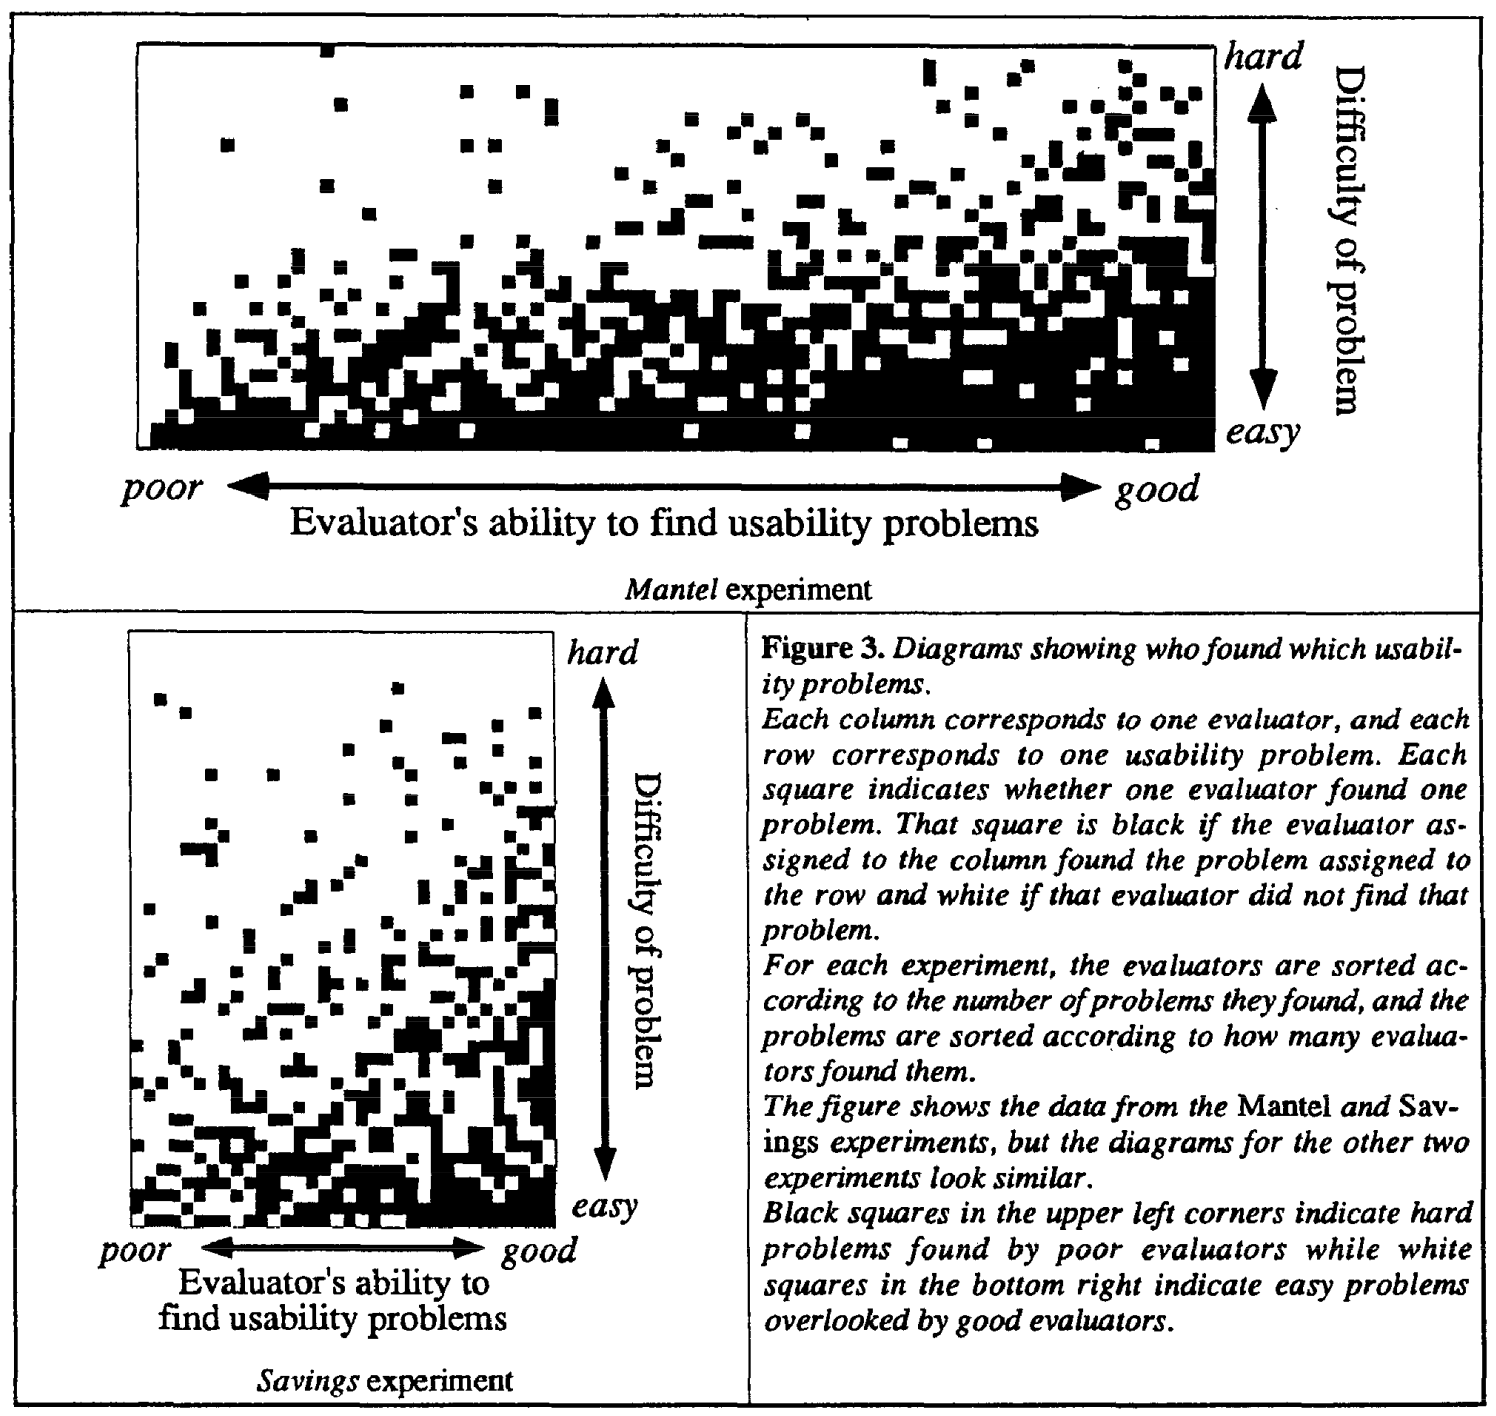
\includegraphics[width=0.8\linewidth]{performance-evaluators}
  \caption{1990 \citeauthor{heureval1990} empirical test of heuristic evaluation\cite{heureval1990}}
  \label{fig:perf}
\end{figure*}

First, as this is a very non-formal and subjective form of evaluation, an evaluator simply looking at an interface or a specification does not see many usability problems. In the early empirical test done by \citeauthor{heureval1990}, evaluators performed quite low: Only one-fifth to half of the problems (that were previously identified by the aggregators) were found by a single person. Also, different evaluators perform weaker or stronger on certain issue categories.
On the other hand, this may be tackled well by multiplying the number of evaluators. Molich and Nielsen also analyse the performing of multiple evaluators, as can be seen in figure ~\ref{fig:perf}. They conclude that 3-5 is an optimal number of evaluators, which is comparably small for a usability evaluation method.

Second, heuristic evaluation tends to discover potential problems rather than actual problems. Following \citeauthor{howtoeval2020}, "problems identified by evaluators can often be false alarms". On the contrary, this may be (to a degree) inevitable using a not-so-empirical usability analysis. This problem may be amplified by the "unpredictable nature" of intelligent systems.

Third, the choice of heuristic is important but difficult. To measure how effective a certain set of heuristics is, one would have to conduct another study like \cite{enhanceheuristics1994}, where the original set of heuristics where refined based on empirical data.

\section{Evaluation of interactive machine learning}

\subsection{New heuristics by \citeauthor{imlheur2018}}

There have been adaptations and redevelopments of the original set of heuristics. Similar to the special nature of many software domains like groupware\cite{groupwareheur2001}, ambient displays, interactive television, et cetera, \citeauthor{imlheur2018} note "how IML challenges many of the assumptions of usability that the original heuristics were meant to address"\cite{imlheur2018}. They developed the below ten new heuristics for IML, structured into three categories:

\subsubsection{Model Input}
The most important aspect of IML is giving the user the ability to influence the model. This is done by reading user input in the first place.
\begin{enumerate}
    \item "Enable the user to steer the model" \\
    \item "Enable the user to provide concept improving feedback" \\
    \item "Capture intent rather than input"\cite{imlheur2018} \\
\end{enumerate}

\subsubsection{User Feedback}
Also very important is the ability to give meaningful feedback to the user. Only this way, the user will know if the model improved at all, and what user actions are needed in the first place.
\begin{enumerate}
    \setcounter{enumi}{3}
    \item "Support user assessment of model quality" \\
    \item "Provide instance-based explanations to the user" \\
    \item "Support rich, natural feedback"\cite{imlheur2018} \\
\end{enumerate}

\subsubsection{Interaction Design}
This guideline category requires the program to design the interaction so that an effective loop of user-to-program and program-to-user feedback emerges.
\begin{enumerate}
    \setcounter{enumi}{6}
    \item "Make interactions and constraints explicit" \\
    \item "Promote trial-and-error based model exploration" \\
    \item "Error prevention" \\
    \item "Help and documentation"\cite{imlheur2018} \\
\end{enumerate}

The authors state, "the specific interpretation and relative importance of these heuris-
tics are likely to vary depending on the level of involvement expected
of the user and on the complexity of the required functionality."\cite{imlheur2018}

\subsection{Execution of the recent HE application}
As IML approach, \citeauthor{imlheur2018} implement two algorithms for decision trees and then examine how well they perform within a heuristic evaluation. They state "it  is  clear  from  our  evaluations that a classification algorithm must get under the 10-20  second  barrier  in  producing  a  new  classification" and "when creating a new perceptual interface it  is  not  classification  time  that  is  the  real  issue. The important issue is designer time."

So \citeauthor{imlheur2018} can confine the list of feasible algorithms, eliminating "slower algorithms such as neural nets or nearest-neighbor."

"We   have   implemented   two   algorithms,   which   employ   different   division   techniques.   These   two   algorithms   also   represent  the  two  approaches  of  longer  training  time  with  better  generalization  vs.  shorter  training  time  with  poorer  generalization. The first strategy slightly reduces interactivity and  relies  more  on  learning  performance.    The  second  relies  on  speed  and  interactivity.    The  two  strategies  are  Center  Weighted (CW) and Mean Split (MS)."\cite{imlheur2018}

\begin{figure}
    \centering
    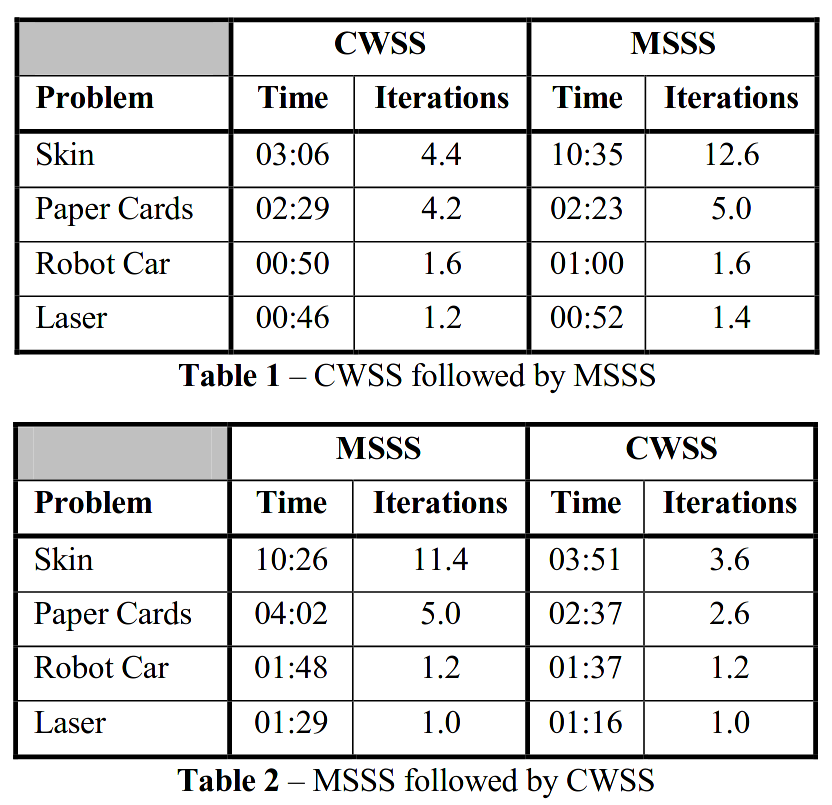
\includegraphics{cwss-vs-msss}
    \caption{Two Decision tree approaches and times a classifier was built during \citeauthor{imlheur2018}'s experiment}
    \label{fig:cwss-vs-msss}
\end{figure}

\begin{figure}
    \centering
    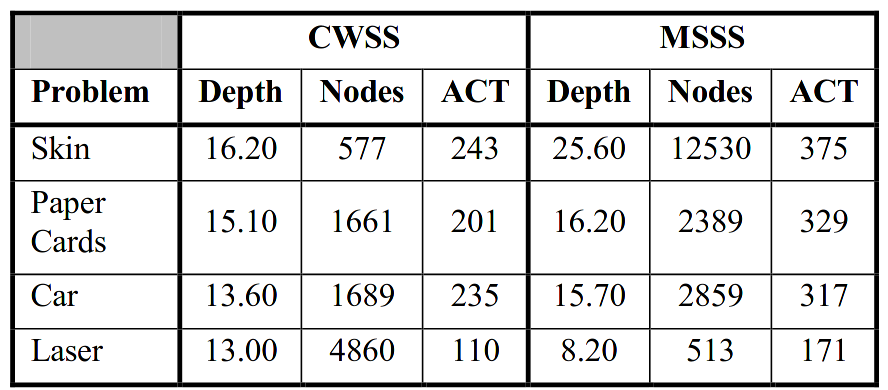
\includegraphics{act}
    \caption{Tree structures and average classification (ACT) time in milliseconds~\cite{imlheur2018}}
    \label{fig:act}
\end{figure}

Figure \ref{fig:cwss-vs-msss} shows that the Center Weight algorithm was faster in building classifiers, and figure \ref{fig:act} shows that it was also faster in classifying. Although Mean Split is quicker in building classifiers, users had to build more often, because the approach was less accurate, thus needing more training data to get acceptable results.

\subsection{Evaluation of the evaluation}
It is important to gather insights in the performance of a method. In the starting time of the heuristic evaluation, there were experiments to measure the effectiveness of the method and certain sets of heuristics (like stated before).

Unfortunately, neither the method nor the newly developed heuristics seem to have been empirically tested in the field of interactive machine learning. Also, literature does not know other attempts to update the Heuristic Evaluation to IML, so the previously mentioned heuristics set by \citeauthor{imlheur2018} cannot be compared to similar work. Thus, the significance and meaningfulness of the newly developed heuristics is limited. It seems this field of research is underdeveloped and has to be extended.

\section{Conclusion}
The heuristic evaluation appears as a valid method for many different types of software, due to its basic nature. It has not to deal with the inner modes of operation, and can be applied also to interactive machine learning systems. The adjustments needed are confined to the generation of a new set of heuristics, which is not unusual for heuristic evaluations.

%%
%% The next two lines define the bibliography style to be used, and
%% the bibliography file.
\bibliographystyle{ACM-Reference-Format}
\bibliography{sample-base}

\end{document}
\endinput